In this chapter we will take a look at mathematical models that describe our quadcopter system.

\section{BLDC Motor}
The mathematical model of a BLDC motor is is many ways similar to the one of a conventional DC motor. The main difference is represented by the added phases which affect the resistive and inductive components of the BLDC arrangement.

Therefore, we will start of by describing the mathematical modelling of a DC motor and then change it to fit the BLDC motor.

Figure \label{electromech} illustrates a DC electromechanical system.

\begin{figure}[H]
  \centering
    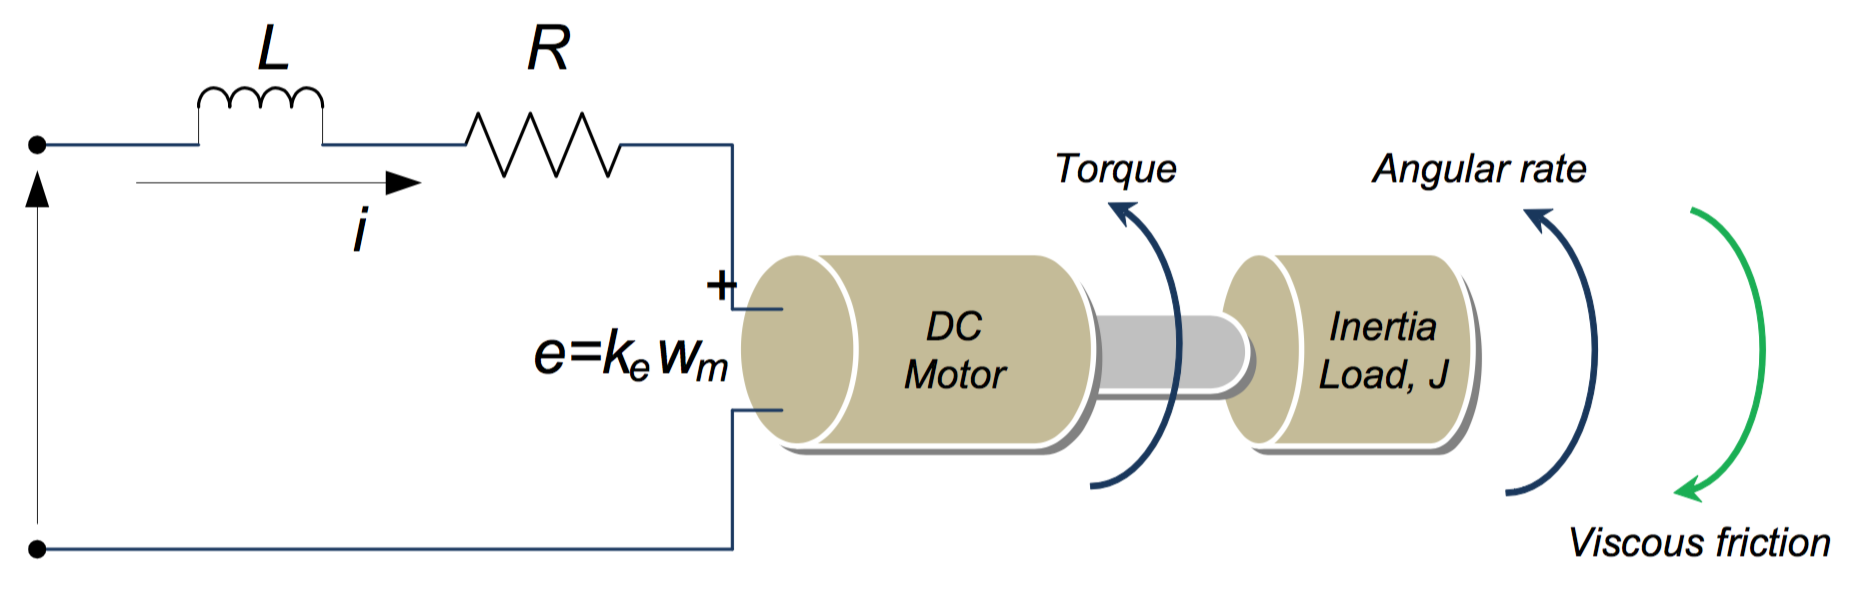
\includegraphics[width=0.9\textwidth]{images/electromech.png}
	\caption{Typical DC electromechanical system}
	\label{electromech}
\end{figure}

The components of the electrical circuit are the armature resistance - R, the armature inductance - L and the back EMF - e. By applying KVL, we obtain:

\begin{equation}
\label{1}
	V_{s}=Ri+L\frac{di}{dt}+e
\end{equation}

where $V_{s}$ - DC source voltage and $i$ - armature current.

Moving on to the mechanical part, further equations can be written using Newton's second law of motion:

\begin{equation}
\label{2}
	J\frac{d\omega_{m}}{dt}=\Sigma{T_{i}}
\end{equation}

\begin{equation}
\label{3}
	T_{e}=k_{f}+J\frac{d\omega_{m}}{dt}+T_{L}
\end{equation}

where $T_{e}$ - electrical torque, $k_{f}$ - friction constant, $J$ - rotor inertia, $\omega_{m}$ - angular velocity and $T_{L}$ - load torque.

The back EMF and the electrical torque can be described as:

\begin{equation}
\label{4}
	T_{e}=k_{t}\omega_{m}
\end{equation}

\begin{equation}
\label{5}
	e=k_{e}\omega_{m}
\end{equation}

where $k_{e}$ - back EMF constant and $k_{t}$ - torque constant.

Rewriting equations \ref{1} and \ref{2} gives:

\begin{equation}
\label{6}
	\frac{di}{dt}=-i\frac{R}{L}-\frac{k_{e}}{L}\omega_{m}+\frac{1}{L}V_{s}
\end{equation}

\begin{equation}
\label{7}
	\frac{d\omega_{m}}{dt}=i\frac{k_{t}}{J}-\frac{k_{f}}{J}\omega_{m}+\frac{1}{J}T_{L}
\end{equation}

Taking the Laplace transform of \ref{6} and \ref{7} yields:

\begin{equation}
\label{8}
	si=i\frac{R}{L}-\frac{k_{e}}{L}\omega_{m}+\frac{1}{L}V_{s}
\end{equation}

\begin{equation}
\label{9}
	s\omega_{m}=i\frac{k_{t}}{J}-\frac{k_{f}}{J}\omega_{m}+\frac{1}{J}T_{L}
\end{equation}

The next equation is obtained by substituting i from equation \ref{9} into \ref{8}.

\begin{equation}
\label{10}
	(\frac{s\omega_{m}+\frac{k_{f}}{J}\omega_{m}-\frac{1}{J}T_{L}}{\frac{k_{t}}{J}})(s+\frac{R}{L})=-\frac{k_{e}}{L}\omega_{m}+\frac{1}{L}V_{s}
\end{equation}  

Assuming there is no load, equation \ref{10} can be rewritten as:

\begin{equation}
\label{11}
	\lbrace{(\frac{s^{2}J}{k_{t}}+\frac{sk_{f}}{k_{t}}+\frac{sRJ}{k_{t}L}+\frac{k_{f}R}{k_{t}L})+\frac{k_{e}}{L}}\rbrace\omega_{m}=\frac{1}{L}V_{s}
\end{equation}

Solving \ref{11} gives:

\begin{equation}
\label{12}
	V_{s}=\frac{s^{2}JL+sk_{f}L+sRJ+k_{f}R+k_{e}k_{t}}{k_{t}}\omega_{m}
\end{equation} 

The transfer function can be obtained as the ratio between the angular velocity $\omega_{m}$ and the source voltage $V_{s}$:

\begin{equation}
\label{13}
	G_{s}=\frac{\omega_{m}}{V_{s}}=\frac{k_{t}}{s^{2}JL+(RJ+k_{f}L)s+k_{f}R+k_{e}k_{t}}
\end{equation} 

Considering that $k_{f}$ tends to zero, the transsfer function can finally be  written as:

\begin{equation}
\label{14}
	G_{s}=\frac{\omega_{m}}{V_{s}}=\frac{k_{t}}{s^{2}JL+RJs+k_{e}k_{t}}
\end{equation} 

In order to obtain the mechanical and electrical time constants, we will need to manipulate equation \ref{14}, which gives:

\begin{equation}
\label{15}
	G_{s}=\frac{\frac{1}{k_{e}}}{\frac{RJ}{k_{e}k_{t}}\frac{L}{R}s^{2}+\frac{RJ}{k_{e}k_{t}}s+1}
\end{equation}

where the mechanical time constant is:

\begin{equation}
\label{16}
	\tau_{m}=\frac{RJ}{k_{e}k_{t}}
\end{equation}

and the electrical time constant is:

\begin{equation}
\label{17}
	\tau_{e}=\frac{L}{R}
\end{equation}

Therefore, substituting equations \ref{16} and \ref{17} into equation \ref{15} yields:

\begin{equation}
\label{18}
	G_{s}=\frac{\frac{1}{k_{e}}}{\tau_{m}\tau_{e}s^{2}+\tau_{m}s+1}
\end{equation}

Equations \ref{15} - \ref{17} will now be changed in order to fit a BLDC motor. Therefore, they will become:

\begin{equation}
\label{19}
	\tau_{m}=\Sigma{\frac{RJ}{k_{e}k_{t}}}=\frac{J\Sigma{R}}{k_{e}k_{t}}
\end{equation}

\begin{equation}
\label{20}
	\tau_{e}=\Sigma{\frac{L}{R}}=\frac{L}{\Sigma{R}}
\end{equation}

Having a symmetrical arrangement and a three phase motor, the constants will finally be:

\begin{equation}
\label{21}
	\tau_{m}=\frac{J3R}{k_{e}k_{t}}
\end{equation}

\begin{equation}
\label{22}
	\tau_{e}=\frac{L}{3R}
\end{equation}

Taking into account the phase effects, $\tau_{m}$ will be rewritten as:

\begin{equation}
\label{23}
	\tau_{m}=\frac{J3R_{\phi}}{k_{e}k_{t}}
\end{equation}

with $k_{e}$ now being the phase value of the back EMF voltage time constant described by:

\begin{equation}
\label{24}
	k_{e}=k_{e(L-L)}/\sqrt{3}
\end{equation}

A relationship between $k_{e}$ - electrical torque and $k_{t}$ - torque constant is found in equation \ref{25}by using the electrical power and mechanical power formulas.

\begin{equation}
\label{25}
	k_{e}=k_{t}\times0.0605
\end{equation}

The next step in coming up with a final transfer function for our motor is to find $\tau_{m}$ and $\tau_{e}$, which are functions of $k_{e}$, $k_{t}$, $R_{\phi}$, J and L. 

A numerical value for $k_{e}$ can be obtained using equation \ref{24}:

\begin{equation}
\label{26}
	k_{e}=\frac{11.1}{1.73}=6.416
\end{equation}

Since $k_{t}$ is a function of $k_{e}$, its numerical value can also be found using equation \ref{25}:

\begin{equation}
\label{27}
	k_{t}=\frac{6.416}{0.0605}=106.04
\end{equation}

For $R_{\phi}$, we have to measure the line-to-line resistance (between any two wires of the motor) and divide the result by 2 in order to get its value.

experiments on J and L / take them from other reports 

\clearpage

\section{Quadcopter Dynamics}

To start describing drone's dynamics, we illustrate two frames - the inertial frame, which is defined by the ground, where the negative $z$ direction shows represents gravity and the body frame. In the body frame, the motor axes point in the positive $z$ direction and the arms point in the $x$ and $y$ directions. These two frames can be seen in figure \ref{frames}.

\begin{figure}[H]
  \centering
    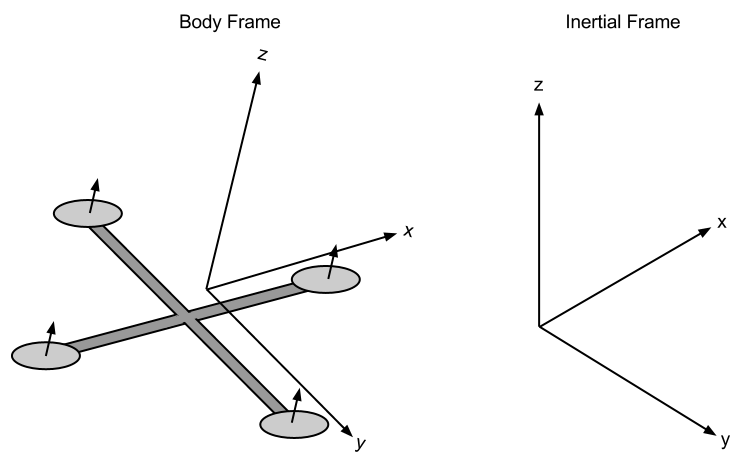
\includegraphics[width=1\textwidth]{images/frames.png}
	\caption{Quadcopter Body Frame and Inertial Frame}
	\label{frames}
\end{figure}

\section{Kinematics}

The drone's position in inertial frame is defined as $x = (x,y,z)^T$. Similarly, the velocity is $\dot{x} = (\dot{x},\dot{y},\dot{z})^T$. In the body frame, we have the roll, pitch and yaw angles given to be $\theta = (\phi,\theta,\Psi)^T$. Then, the angular velocities are equal to $\dot{\theta} = (\dot{\phi},\dot{\theta},\dot{\psi})^T$.
It should be noted that the angular velocity vector $\omega$ is not equal to the angular velocity $\dot{\theta}$ itself. It is possible to convert angular velocity into angular velocity vector using the following expression:
\begin{equation}
\label{mmKinematics1}
\omega = \begin{bmatrix}
       	1		& 0 		& -s_\theta			\\
       	0 		& c_\phi 	& c_\theta s_\phi 	\\
      	0       & -s_\phi 	& c_\theta c_\phi 	\\
\end{bmatrix} \dot{\theta}
\end{equation}
where $\omega$ is the angular velocity vector.

Both frames can be related using a rotation matrix $R$, which goes from one frame to another. The matrix is obtained using the ZYZ Euler angle conventions.
\begin{equation}
\label{mmKinematics2}
R = \begin{bmatrix}
       	c_\phi c_\psi - c_\theta s_\phi s_\psi		& -c_\psi s_\phi - c_\phi c_\theta s_\psi 	& s_\theta s_\psi			\\
       	c_\theta c_\psi s_\phi + c_\phi s_\psi 		& c_\phi c_\theta c_\psi - s_\phi s_\psi 	& -c_\psi s_\theta 			\\
      	s_\phi s_\theta       						& c_\phi s_\theta 								& c_\theta 					\\
\end{bmatrix}
\end{equation}
Therefore, a vector $\overrightarrow{v}$ in the body frame can be defined as $R\overrightarrow{v}$ in the inertial frame.

\section{Motor Dynamics}
A brushless motor produces torque given by equation \ref{mmMotor1}.
\begin{equation}
\label{mmMotor1}
	\tau = K_t(I-I_0)
\end{equation}

Here, $\tau$ is the torque, $I$ is the input current, $K_t$ is the constant describing torque proportionality and $I_0$ is the no-load current.

The voltage on the motor is the sum of a resistive loss and the Back-EMF, giving equation \ref{mmMotor2}.
\begin{equation}
\label{mmMotor2}
	V = IR_m + K_e\omega
\end{equation}
where $V$ is the voltage across the motor, $R_m$ is the motor resistance, $\omega$ is the angular velocity and $K_e$ is a constant, describing the back-EMF generated per $RPM$.
We can then combine equations \ref{mmMotor1} and \ref{mmMotor2} and put them into the power equation, to get a new equation \ref{mmMotor3}.
\begin{equation}
\label{mmMotor3}
	P = IV = \frac{(\tau + K_tI_0)(K_tI_0R_m + \tau R_m + K_tK_e\omega)}{K_t^2}
\end{equation}

To help simplify the model, we can assume that the motor resistance is very small and therefore can be disregarded. This gives us a new power equation \ref{mmMotor4}.
\begin{equation}
\label{mmMotor4}
	P \approx \frac{(\tau + K_tI_0)K_e\omega}{K_t}
\end{equation}

We can also, for the purposes of simplifying the model, assume that $K_tI_0\ll \tau$. This is a reasonable assumption due to the fact that $I_0$ describes the current with no load on the motor and is usually a small number. Based on this, we can then obtain the final equation \ref{mmMotor5} for power.
\begin{equation}
\label{mmMotor5}
	P \approx \frac{K_e}{K_t}\tau \omega
\end{equation}

\section{Forces}

From the conservation of energy, it is known that the energy that the motor expends during some period of time is equal to the force generated by the propeller multiplied by the distance the it displaces moves, given by the equation \ref{mmMotor6}.
\begin{equation}
\label{mmMotor6}
	P\times dt = F\times dx
\end{equation}
We can then say that the power is also equal to the thrust multiplied by the air velocity, as seen in equation \ref{mmMotor7}.
\begin{equation}
\label{mmMotor7}
	P = F\frac{dt}{dx} = Tv_h
\end{equation}
Here - $T$ is the thrust and $v_h$ is the air velocity. Since the model is describing a hovering quadcopter in a closed area, only $v_h$ is an acting velocity (i.e. vehicle speed has no effect and free stream velocity is equal to zero).

Momentum theory gives equation \ref{mmMotor8}, for the hover velocity $v_h$.
\begin{equation}
\label{mmMotor8}
	v_h = \sqrt{\frac{T}{2\rho A}}
\end{equation}

where $A$ is the area swept out by the blade and $\rho$ is the air density.
In the case of this model, $\tau$ is proportional to thrust $T$ by a constant $K_\tau$. Keeping this in mind, we can now use the simplified power equation \ref{mmMotor5} and derive a new equation \ref{mmMotor9}.
\begin{equation}
\label{mmMotor9}
 	P = \frac{K_e}{K_t}\tau \omega = \frac{K_eK_\tau }{K_t}T\omega = \frac{F^{\frac{3}{2}}} {\sqrt{2\rho A}}
\end{equation}

Solving for thrust $T$, we can derive a new equation \ref{mmMotor10}.
\begin{equation}
\label{mmMotor10}
 	T = (\frac{K_eK_\tau \sqrt{2\rho A}}{K_t}\omega)^2 = k\omega ^2
\end{equation}

where $k$ is a constant, describing all other constants used in the equation.

The final equation \ref{mmMotor10} now describes the thrust $T$ generated by the motor with angular velocity $\omega$ as an input.

We can now sum the thrust over all motors. This sum is then given by
\begin{equation}
\label{mmMotor11}
 	T_B = \displaystyle\sum_{i=1}^{4} T_i = k 	
 	\begin{bmatrix}
 	0 					\\
 	0 					\\
 	\sum \omega _i^2	\\ 
 	\end{bmatrix}	
\end{equation}

We can model a simplified version of fluid friction as a force proportional to the linear velocity in each direction. Then, drag forces will have another force term in their model:
\begin{equation}
\label{mmMotor12}
 	F_D = \begin{bmatrix}
 	-k_d\dot{x}	\\
 	-k_d\dot{y} \\
 	-k_d\dot{z} \\ 
 	\end{bmatrix}	
\end{equation}

\section{Torques}
Every motor produces some torque about the z axis in the body frame. This torque is the requirement for the torque produces by the motor to keep the motor providing thrust by spinning the propeller. The spinning propeller overcomes frictional forces and creates angular acceleration.
The frictional force is acquired from fluid dynamics as follows:
\begin{equation}
\label{mmTorque1}
 	F_D = \frac{1}{2}\rho C_DAv^2
\end{equation}
Here, $\rho$ is the fluid density, $A$ is the propeller cross-section area, $C_D$ is a dimensionless constant.
We can then derive an equation for torque produced due to drag force:
\begin{equation}
\label{mmTorque2}
	\tau _D = \frac{1}{2}R\rho C_DAv^2 = \frac{1}{2}R\rho C_DA(\omega R)^2 = b\omega ^2
\end{equation}
where $b$ is an appropriately dimensioned constant.
While we assume that force all of the force is applied at the top of the propeller, our only concern is that the drag torque is proportional to the angular velocity.
Torque for the $i^{th}$ motor about the $z$ axis can then be described as follows:
\begin{equation}
\label{mmTorque3}
	\tau _z = (-1)^{i+1}b\omega ^2 + I_M\dot{\omega}
\end{equation}
Here, $I_M$ is the moment of inertia about the $z$ axis of the motor, $\dot{\omega}$ is the angular acceleration of the propeller and the term $(-1)^{i+1}$ is describing the direction of rotation of the $i^{th}$ motor (i.e. whether it is spinning clockwise or counter-clockwise).
Since in a steady state there is no acceleration, we can say that $\dot{\omega} \approx 0$ and drop the term. The simplified equation then becomes
\begin{equation}
\label{mmTorque4}
	\tau _z = (-1)^{i+1}b\omega ^2
\end{equation}
Then, we can derive an equation for total torque about the $z$ axis.
\begin{equation}
\label{mmTorque5}
	\tau _\psi = b(\omega _1^2 - \omega _2^2 + \omega _3^2 - \omega _4 ^2)
\end{equation}
If we select motors $1$ and $3$ to be on the roll axis, we can the following roll torque equation:
\begin{equation}
\label{mmTorque6}
	\tau _\phi = \sum r\times T = L(k\omega _1^2 - k\omega _3^2) = Lk(\omega _1^2 - \omega _3^2)
\end{equation}
Here, $L$ defines the distance from the propeller to the centre of the quadcopter, assuming all motors are placed at equal distances.
Similarly, we can obtain the pitch torque for the other two motors:
\begin{equation}
\label{mmTorque7}
	\tau _\theta = Lk(\omega _2^2 - \omega _4^2)
\end{equation}

A matrix describing all torques in the body frame can be seen in equation \ref{mmTorque8}.
\begin{equation}
\label{mmTorque8}
 	\tau _B = \begin{bmatrix}
 	Lk(\omega _1^2 - \omega _3^2)								\\
 	Lk(\omega _2^2 - \omega _4^2) 								\\
 	b(\omega _1^2 - \omega _2^2 + \omega _3^2 - \omega _4 ^2) 	\\ 
 	\end{bmatrix}	
\end{equation}

\section{Equations of Motion}
Quadcopter's acceleration in the inertial frame is caused by gravity, thrust and linear fircion. We can obtain thrust vector in the inertial frame through the use of rotation matrix $R$ to map thrust vector from one frame to the other.
Linear motion can then be described by equation \ref{mmMotion1}.
\begin{equation}
\label{mmMotion1}
 	m\ddot{x} = \begin{bmatrix}
 	0	\\
 	0	\\
 	-mg	\\ 
 	\end{bmatrix}	
\end{equation}
Since we prefer to express rotations about the centre of the vehicle instead of about inertial centre, it is more reasonable to use rotational equations of motion in body frame. We can derive these equations from Euler’s equations for rigid body dynamics. The equation \ref{mmMotion2} is expressed in vector form.
\begin{equation}
\label{mmMotion2}
	I\dot{\omega} + \omega \times (I\omega ) = \tau
\end{equation}
It can then be rewritten as equation \ref{mmMotion3}.
\begin{equation}
\label{mmMotion3}
 	\dot{\omega} = \begin{bmatrix}
 	\dot{\omega _x}	\\
 	\dot{\omega _y}	\\
 	\dot{\omega _z}	\\ 
 	\end{bmatrix} = I^{-1}(\tau - \omega \times (I\omega ))
\end{equation}
A drone model can be understood as two lines crossed together at origin with a point mass as motors at the end of each line. From this, we can derive a diagonal inertia matrix \ref{mmMotion4}.
\begin{equation}
\label{mmMotion4}
 	I = \begin{bmatrix}
 	I_{xx}	& 0 		& 0			\\
 	0 		& I_{yy}	& 0			\\
 	0 		& 0 		& I_{zz}	\\ 
 	\end{bmatrix} = I^{-1}(\tau - \omega \times (I\omega ))
\end{equation}
Taking everything into consideration, a final result for the rotational equations of motion in body frame are given as equation \ref{mmMotion5}.
\begin{equation}
\label{mmMotion5}
 	\dot{\omega} = \begin{bmatrix}
 	\tau _\phi I_{xx}^{-1}		\\
 	\tau _\theta I_{yy}^{-1}	\\
 	\tau _\psi I_{zz}^{-1}		\\ 
 	\end{bmatrix} - \begin{bmatrix}
 	\frac{I_{yy}-I{zz}}{I_{xx}}\omega _y\omega _z	\\
 	\frac{I_{zz}-I{xx}}{I_{yy}}\omega _x\omega _z	\\
 	\frac{I_{xx}-I{yy}}{I_{zz}}\omega _x\omega _y	\\ 
 	\end{bmatrix}
\end{equation}

\section{Control}
Having a mathematical model of the system makes the development of controller easier. With only input being the angular velocities of each motor, we can write the system as a first order differential equation in state space.

\begin{equation}
\label{mmControl1}
	\dot{x_1} = x_2	\\
\end{equation}
\begin{equation}
\label{mmControl2}
	\dot{x_2} = \begin{bmatrix}
 	0	\\
 	0	\\
 	-g 	\\
 	\end{bmatrix} + \frac{1}{m}RT_B + \frac{1}{m}F_D \\
\end{equation}
\begin{equation}
\label{mmControl3} 	
 	\dot{x_3} = \begin{bmatrix}
       	1		& 0 		& -s_\theta			\\
       	0 		& c_\phi 	& c_\theta s_\phi 	\\
      	0       & -s_\phi 	& c_\theta c_\phi 	\\
	\end{bmatrix}^{-1}x_4 \\
\end{equation}
\begin{equation}
\label{mmControl4}	
	\dot{x_4} = \begin{bmatrix}
 	\tau _\phi I_{xx}^{-1}		\\
 	\tau _\theta I_{yy}^{-1}	\\
 	\tau _\psi I_{zz}^{-1}		\\ 
 	\end{bmatrix} - \begin{bmatrix}
 	\frac{I_{yy}-I{zz}}{I_{xx}}\omega _y\omega _z	\\
 	\frac{I_{zz}-I{xx}}{I_{yy}}\omega _x\omega _z	\\
 	\frac{I_{xx}-I{yy}}{I_{zz}}\omega _x\omega _y	\\ 
 	\end{bmatrix}
 \end{equation}
Here, $x_1$ is the position of the vehicle in space, $x_2$ is the drone's linear velocity, $x_3$ denotes the angles of pitch, roll and yaw and $x_4$ shows the angular velocity vector.